\documentclass[../../main.tex]{subfiles}
\begin{document}

{\bf[解]}

\begin{figure}[htb]
  \centering
  \tdplotsetmaincoords{65}{115}
  \begin{tikzpicture}[tdplot_main_coords, scale=2.5, >=stealth, every node/.style={font=\small}]
    % 図ではt=0.75とした代表例を描く．
    \coordinate (O) at (0,0,0);
    \coordinate (A) at (1,0,1);
    \coordinate (P) at (0,0.75,0.4375);
    \draw[->,thick] (O) -- (1.6,0,0) node[below left] {$x$};
    \draw[->,thick] (0,-1.25,0) -- (0,1.55,0) node[right] {$y$};
    \draw[->,thick] (0,0,-0.65) -- (0,0,1.55) node[above] {$z$};
    \node[below left] at (O) {$O$};
    \draw[very thick,blue!85!black,domain=-1.2:1.2,samples=81,variable=\u]
    plot (0,\u,{1-\u*\u});
    \draw[dashed,gray!60] (A) -- (1,0,0);
    \draw[dashed,gray!60] (0,0,1) -- (A);
    \draw[dashed,gray!60] (P) -- (0,0.75,0);
    \draw[->,very thick,red!85!black] (A) -- (P)
    node[midway,above] {$\overrightarrow{AP}$};
    \fill[red!85!black] (A) circle (0.7pt) node[left] {$A(1,0,1)$};
    \fill[blue!85!black] (P) circle (0.7pt) node[above right] {$P(0,t,1-t^2)$};
    \node[below] at (0,0.75,0) {$t$};
    \node[above left] at (0,0,1) {$1$};
    \node[below] at (1,0,0) {$1$};
    \node[blue!85!black,below left] at (0,-1.2,-0.44) {$z=1-y^2$};
  \end{tikzpicture}
  \caption{$yz$平面上の放物線とベクトル$\overrightarrow{AP}$（$0<t<1$の例）}
  \label{fig:utokyo1987q4_parabola_AP}
\end{figure}

題意より$P$が$yz$平面，すなわち$x=0$上の放物線$z=1-y^2$にあるから，パラメータ$t$を用いて$P(0,t,1-t^2)$とおく．また点$A(1,0,1)$だからベクトル$\vec{a}=(1,0,1)$とする．題意の直線$AP$の方向ベクトルは$\vec{l}$は$\vec{l}=(-1,t,-t^2)$であるから，この直線上の点$X$は
\begin{align}
  & l:\overrightarrow{OX}=\vec{a}+p\vec{l} \\
  & (x,y,z) = (1,0,1) + p(-1,t,-t^2)
\end{align}
と書ける．

$x=k(0\le k\le 1)$とすると$1-p = k \therefore p=1-k$だから，$X$の座標は
$X\left(k，(1-k)t,1-(1-k)t^2\right)$である．
したがって，直線$AP$を$x$軸周りに回転した軌跡の$x=k$での切断面は，$X$を$x$軸周りに回転した円に等しく，下図のようになる．

\begin{figure}[htb]
  \centering
  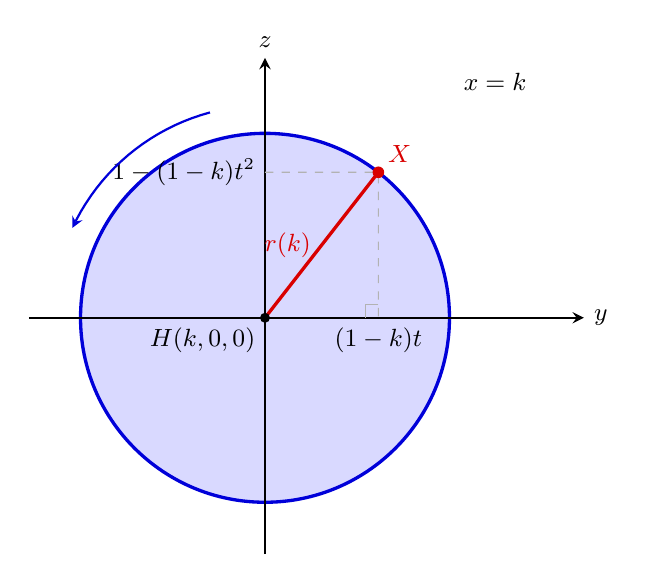
\begin{tikzpicture}[scale=3, >=stealth, every node/.style={font=\small}]
    % 図ではk=0.4，t=0.8とした代表例を描く．
    \coordinate (H) at (0,0);
    \coordinate (X) at (0.48,0.616);
    \pgfmathsetmacro{\sectionRadius}{sqrt(0.48^2+0.616^2)}
    \fill[blue!15] (H) circle (\sectionRadius);
    \draw[very thick,blue!85!black] (H) circle (\sectionRadius);
    \draw[->,thick] (-1,0) -- (1.35,0) node[right] {$y$};
    \draw[->,thick] (0,-1) -- (0,1.10) node[above] {$z$};
    \draw[dashed,gray!60] (0,0.616) -- (X) -- (0.48,0);
    \draw[very thick,red!85!black] (H) -- (X)
    node[midway,left] {$r(k)$};
    \fill (H) circle (0.6pt) node[below left] {$H(k,0,0)$};
    \fill[red!85!black] (X) circle (0.7pt) node[above right] {$X$};
    \node[below] at (0.48,0) {$(1-k)t$};
    \node[left] at (0,0.616) {$1-(1-k)t^2$};
    \draw[gray!60] (0.48,0.055) -- (0.425,0.055) -- (0.425,0);
    \draw[->,thick,blue!85!black,domain=105:155,samples=21]
    plot ({0.9*cos(\x)},{0.9*sin(\x)});
    \node[above right] at (0.80,0.92) {$x=k$};
  \end{tikzpicture}
  \caption{平面$x=k$での断面．$X$は$x$軸上の点$H$を中心とする円を描く．}
  \label{fig:utokyo1987q4_section}
\end{figure}

この円の半径$r(k)$は
\begin{align}
  r(k) = \sqrt{\left((1-k)t\right)^2 + \left(1-(1-k)t^2\right)^2}
\end{align}
だから，この平面での断面積$S(k)$は
\begin{align}
  S(k)
  &= \pi r^2(k) \\
  &= \pi\left\{\left((1-k)t\right)^2+\left(1-(1-k)t^2\right)^2\right\} \\
  &= \pi\left\{1-2t^2(1-k)+(t^4+t^2)(1-k)^2\right\} \\
\end{align}
となる．よって領域の体積$V$は
\begin{align}
  V&=\int_0^1S(k)dk \\
  &=\pi\left[k+t^2(1-k)^2-\dfrac{1}{3}(t^4+t^2)(1-k)^3\right]_0^1 \\
  &=\pi(1-t^2+\dfrac{1}{3}(t^4+t^2)) \\
  &=\pi\left(\dfrac{1}{3}t^4-\dfrac{2}{3}t^2+1\right) \\
  &=\dfrac{\pi}{3}\left(t^2-1\right)^2+\dfrac{2\pi}{3} \cdots\text{(答)}
\end{align}
である．

よって$V$の最小値は$t=\pm1$のときの
\begin{align}
  \min V=\dfrac{2}{3}\pi\cdots\text{(答)}
\end{align}
である．
\newpage
\end{document}
